% Options for packages loaded elsewhere
\PassOptionsToPackage{unicode}{hyperref}
\PassOptionsToPackage{hyphens}{url}
%
\documentclass[
]{article}
\usepackage{amsmath,amssymb}
\usepackage{lmodern}
\usepackage{iftex}
\ifPDFTeX
  \usepackage[T1]{fontenc}
  \usepackage[utf8]{inputenc}
  \usepackage{textcomp} % provide euro and other symbols
\else % if luatex or xetex
  \usepackage{unicode-math}
  \defaultfontfeatures{Scale=MatchLowercase}
  \defaultfontfeatures[\rmfamily]{Ligatures=TeX,Scale=1}
\fi
% Use upquote if available, for straight quotes in verbatim environments
\IfFileExists{upquote.sty}{\usepackage{upquote}}{}
\IfFileExists{microtype.sty}{% use microtype if available
  \usepackage[]{microtype}
  \UseMicrotypeSet[protrusion]{basicmath} % disable protrusion for tt fonts
}{}
\makeatletter
\@ifundefined{KOMAClassName}{% if non-KOMA class
  \IfFileExists{parskip.sty}{%
    \usepackage{parskip}
  }{% else
    \setlength{\parindent}{0pt}
    \setlength{\parskip}{6pt plus 2pt minus 1pt}}
}{% if KOMA class
  \KOMAoptions{parskip=half}}
\makeatother
\usepackage{xcolor}
\usepackage[margin=1in]{geometry}
\usepackage{longtable,booktabs,array}
\usepackage{calc} % for calculating minipage widths
% Correct order of tables after \paragraph or \subparagraph
\usepackage{etoolbox}
\makeatletter
\patchcmd\longtable{\par}{\if@noskipsec\mbox{}\fi\par}{}{}
\makeatother
% Allow footnotes in longtable head/foot
\IfFileExists{footnotehyper.sty}{\usepackage{footnotehyper}}{\usepackage{footnote}}
\makesavenoteenv{longtable}
\usepackage{graphicx}
\makeatletter
\def\maxwidth{\ifdim\Gin@nat@width>\linewidth\linewidth\else\Gin@nat@width\fi}
\def\maxheight{\ifdim\Gin@nat@height>\textheight\textheight\else\Gin@nat@height\fi}
\makeatother
% Scale images if necessary, so that they will not overflow the page
% margins by default, and it is still possible to overwrite the defaults
% using explicit options in \includegraphics[width, height, ...]{}
\setkeys{Gin}{width=\maxwidth,height=\maxheight,keepaspectratio}
% Set default figure placement to htbp
\makeatletter
\def\fps@figure{htbp}
\makeatother
\setlength{\emergencystretch}{3em} % prevent overfull lines
\providecommand{\tightlist}{%
  \setlength{\itemsep}{0pt}\setlength{\parskip}{0pt}}
\setcounter{secnumdepth}{5}
\newlength{\cslhangindent}
\setlength{\cslhangindent}{1.5em}
\newlength{\csllabelwidth}
\setlength{\csllabelwidth}{3em}
\newlength{\cslentryspacingunit} % times entry-spacing
\setlength{\cslentryspacingunit}{\parskip}
\newenvironment{CSLReferences}[2] % #1 hanging-ident, #2 entry spacing
 {% don't indent paragraphs
  \setlength{\parindent}{0pt}
  % turn on hanging indent if param 1 is 1
  \ifodd #1
  \let\oldpar\par
  \def\par{\hangindent=\cslhangindent\oldpar}
  \fi
  % set entry spacing
  \setlength{\parskip}{#2\cslentryspacingunit}
 }%
 {}
\usepackage{calc}
\newcommand{\CSLBlock}[1]{#1\hfill\break}
\newcommand{\CSLLeftMargin}[1]{\parbox[t]{\csllabelwidth}{#1}}
\newcommand{\CSLRightInline}[1]{\parbox[t]{\linewidth - \csllabelwidth}{#1}\break}
\newcommand{\CSLIndent}[1]{\hspace{\cslhangindent}#1}
\usepackage{booktabs}
\usepackage{longtable}
\usepackage{array}
\usepackage{multirow}
\usepackage{wrapfig}
\usepackage{float}
\usepackage{colortbl}
\usepackage{pdflscape}
\usepackage{tabu}
\usepackage{threeparttable}
\usepackage{threeparttablex}
\usepackage[normalem]{ulem}
\usepackage{makecell}
\usepackage{xcolor}
\ifLuaTeX
  \usepackage{selnolig}  % disable illegal ligatures
\fi
\IfFileExists{bookmark.sty}{\usepackage{bookmark}}{\usepackage{hyperref}}
\IfFileExists{xurl.sty}{\usepackage{xurl}}{} % add URL line breaks if available
\urlstyle{same} % disable monospaced font for URLs
\hypersetup{
  hidelinks,
  pdfcreator={LaTeX via pandoc}}

\author{}
\date{\vspace{-2.5em}}

\begin{document}

\hypertarget{your-horse-is-a-donkey-identifying-domesticated-equids-from-western-iberia-using-collagen-fingerprinting}{%
\section*{Your horse is a donkey! Identifying domesticated equids from Western Iberia using collagen fingerprinting}\label{your-horse-is-a-donkey-identifying-domesticated-equids-from-western-iberia-using-collagen-fingerprinting}}
\addcontentsline{toc}{section}{Your horse is a donkey! Identifying domesticated equids from Western Iberia using collagen fingerprinting}

\begin{center}
Supplementary Information
\end{center}

The raw data has been uploaded to the following locations for open access:\\

\begin{itemize}
\tightlist
\item
  MS/MS Data:

  \begin{itemize}
  \tightlist
  \item
    DOI: \url{doi:10.25345/C5T727K8H}
  \item
    ProteomeXchange through MassIVE: PXD035509
  \item
    MassIVE Record Number: MSV000089943
  \end{itemize}
\item
  ZooMS Spectra:

  \begin{itemize}
  \tightlist
  \item
    DOI: 10.5281/zenodo.6878868
  \item
    Zenodo Record Number: 6878868
  \end{itemize}
\end{itemize}

Also uploaded with the ZooMS Spectra to Zenodo under the same DOI are:\\
1. Aligned FASTA files for the mature peptides of \(col1 \alpha 1\) and \(col1 \alpha 2\) of all sequences used in the manuscript.

\hypertarget{included-in-this-supplemental-information-pdf}{%
\subsection*{Included in this Supplemental Information PDF}\label{included-in-this-supplemental-information-pdf}}
\addcontentsline{toc}{subsection}{Included in this Supplemental Information PDF}

\hypertarget{supplemental-figures}{%
\subsubsection*{Supplemental Figures}\label{supplemental-figures}}
\addcontentsline{toc}{subsubsection}{Supplemental Figures}

Figure S1: MS/MS examples for the distinguishing chymotryptic peptide in horse and donkey\\

\hypertarget{supplemental-tables}{%
\subsubsection*{Supplemental Tables}\label{supplemental-tables}}
\addcontentsline{toc}{subsubsection}{Supplemental Tables}

Table S1: Sample list of all archaeological and taxonomic reference samples analysed in this study.\\
Table S2: List of published collagen markers for species from the Equidae family.\\
Table S3: Number of proteins in proteome search and coverage of collagen for confirmation search digested with chymotrypsin.

\newpage

\hypertarget{si-figure-1-msms-sequence-identification-of-biomarkers}{%
\subsection*{SI Figure 1: MS/MS Sequence Identification of Biomarkers}\label{si-figure-1-msms-sequence-identification-of-biomarkers}}
\addcontentsline{toc}{subsection}{SI Figure 1: MS/MS Sequence Identification of Biomarkers}

The MS/MS spectra of the peptides for the diagnostic marker COL1A1 991-1018 from horse (LARC.265) and donkey (LARC.1498). Both peptides have 4 proline oxidations.

\hypertarget{horse-mz-2497}{%
\subsubsection*{Horse: m/z 2497}\label{horse-mz-2497}}
\addcontentsline{toc}{subsubsection}{Horse: m/z 2497}

\begin{center}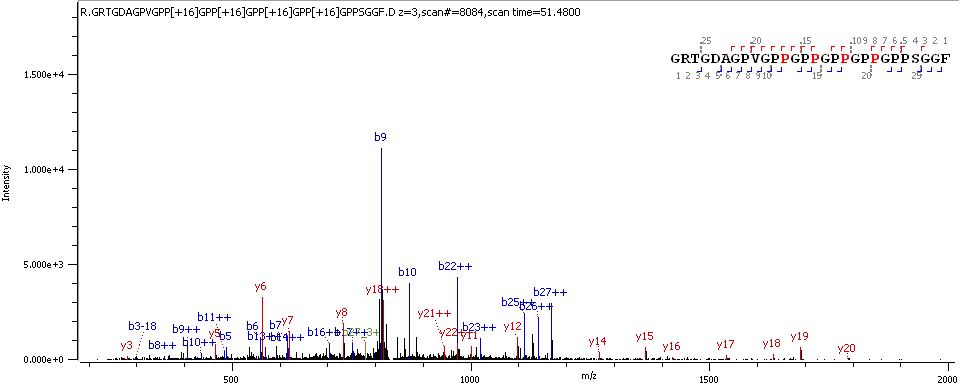
\includegraphics{../img/265-2497} \end{center}

\hypertarget{donkey-mz-2511}{%
\subsubsection*{Donkey m/z 2511}\label{donkey-mz-2511}}
\addcontentsline{toc}{subsubsection}{Donkey m/z 2511}

\begin{center}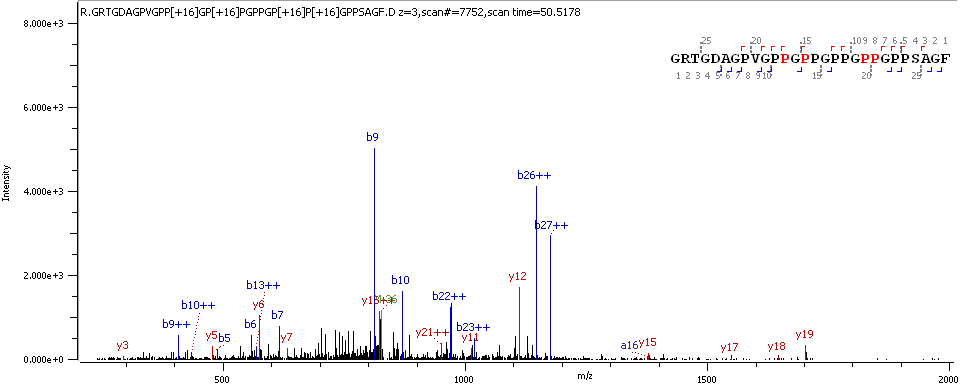
\includegraphics{../img/1498-2511} \end{center}

\newpage

\begin{landscape}\begin{table}

\caption{\label{tab:si1table}Sample list of all archaeological and taxonomic reference samples analysed in this study.}
\centering
\fontsize{7}{9}\selectfont
\begin{tabular}[t]{cccccc>{}c>{}c}
\toprule
Sample ID & Lab Code & Site & Country & Time Period & Skeletal Element & Morphological Id. & ZooMS Id.\\
\midrule
TRAOF100 & HZ145 & Troia & Portugal & Roman & Left Femur & \em{Equus asinus} & \em{Equus asinus}\\
TRAOF101 & HZ146 & Troia & Portugal & Roman & Left Scapula & \em{Equus asinus} & \em{Equus asinus}\\
TRAOF102 & HZ147 & Troia & Portugal & Roman & Mandible & \em{Equus asinus} & \em{Equus asinus}\\
TRAOF104 & HZ149 & Troia & Portugal & Roman & Pelvis & \em{Equus asinus} & \em{Equus asinus}\\
TRAOF105 & HZ150 & Troia & Portugal & Roman & Rib & \em{Equus {\normalfont sp.}} & \em{Equus asinus}\\
TRAOF107 & HZ152 & Troia & Portugal & Roman & Long bone fragment & \em{Equus {\normalfont sp.}} & \em{Equus asinus}\\
RDA.19.EQ1 & HZ156 & Rua do Anjos & Portugal & Roman & Molar & \em{Equus {\normalfont sp.}} & \em{Equus asinus}\\
RDA.19.EQ2 & HZ157 & Rua do Anjos & Portugal & Roman & Molar & \em{Equus {\normalfont sp.}} & \em{Equus caballus}\\
RDA.19.EQ3 & HZ158 & Rua do Anjos & Portugal & Roman & Mandible & \em{Equus {\normalfont sp.}} & \em{Equus caballus}\\
RDA.19.EQ4 & HZ159 & Rua do Anjos & Portugal & Roman & Metapode & \em{Equus {\normalfont sp.}} & \em{Equus caballus}\\
RDA.19.EQ5 & HZ160 & Rua do Anjos & Portugal & Roman & Metapode & \em{Equus {\normalfont sp.}} & \em{Equus caballus}\\
RDA.19.EQ7 & HZ161 & Rua do Anjos & Portugal & Roman & Radius & \em{Equus {\normalfont sp.}} & \em{Equus caballus}\\
RDA.19.EQ8 & HZ162 & Rua do Anjos & Portugal & Roman & Pelvis & \em{Equus {\normalfont sp.}} & \em{Equus caballus}\\
RDA.19.EQ9 & HZ163 & Rua do Anjos & Portugal & Roman & Astragalus & \em{Equus {\normalfont sp.}} & \em{Equus asinus}\\
RDA.19.EQ10 & HZ164 & Rua do Anjos & Portugal & Roman & Femur & \em{Equus {\normalfont sp.}} & \em{Equus caballus}\\
LCB.15.EQ19 & HZ153 & Largo do Coutador & Portugal & Late Antiquity & Metapode & \em{Equus {\normalfont sp.}} & \em{Equus asinus}\\
LCB.15.EQ18 & HZ154 & Largo do Coutador & Portugal & Late Antiquity & Molar & \em{Equus {\normalfont sp.}} & \em{Equus asinus}\\
LCB.15.EQ17 & HZ155 & Largo do Coutador & Portugal & Late Antiquity & Molar & \em{Equus {\normalfont sp.}} & \em{Equus asinus}\\
RNA63EQ11 & HZ165 & Rua Nova do Almada 63 & Portugal & Roman Imperial & Molar & \em{Equus {\normalfont sp.}} & \em{Equus caballus}\\
RNA63EQ12 & HZ166 & Rua Nova do Almada 63 & Portugal & Roman Imperial & Incisor & \em{Equus {\normalfont sp.}} & \em{Equus asinus}\\
BPLX.246 & HZ167 & Banco de Portugal & Portugal & Roman & Cranium & \em{Equus {\normalfont sp.}} & \em{Equus asinus}\\
H4.1070.1 & HZ143 & Los Morrones 11 & Spain & Iron Age & Radius & \em{Equus caballus} & \em{Equus caballus}\\
H4.1070.2 & HZ144 & Los Morrones 12 & Spain & Iron Age & Radius & \em{Equus caballus} & \em{Equus caballus}\\
H4.1075.3 & PHD1075.3 & Los Morrones 11 & Spain & Iron Age & Radius & \em{Equus caballus} & \em{Equus caballus}\\
TRSLOF100 & HZ140 & Torre Sal & Spain & Iberian & Radius & \em{Equus caballus} & \em{Equus caballus}\\
TRSLOF103 & PHDTSOF100 & Torre Sal & Spain & Iberian & Radius & \em{Equus caballus} & \em{Equus caballus}\\
MJV.1 & HZ121 & Horta da Torre & Portugal & Late Roman & Right Radius & \em{Equus caballus} & \em{Equus caballus}\\
MJV.2 & HZ122 & Horta da Torre & Portugal & Late Roman & Right Metacarpus & \em{Equus caballus} & \em{Equus caballus}\\
MJV.3 & HZ123 & Cacela - Po\c{c}o Antigo & Portugal & Late Medieval Islamic & Calcaneum R & \em{Equus {\normalfont sp.}} & \em{Equus caballus}\\
MJV.5 & HZ125 & Cacela - Largo Fortaleza & Portugal & Late Medieval Islamic/Christian & Upper Incisor 1 or 2 R (root) & \em{Equus {\normalfont sp.}} & \em{Equus asinus}\\
MJV.7 & HZ127 & Oficina Senhor Carrilho & Portugal & Medieval Islamic & Metapodial & \em{Equus {\normalfont sp.}} & \em{Equus caballus}\\
MJV.11 & HZ131 & Castillo de Aracena & Spain & Medieval Islamic & Scapula R & \em{Equus {\normalfont sp.}} & \em{Equus caballus}\\
MJV.12 & HZ132 & Castillo de Aracena & Spain & Late Medieval Islamic/Christian & Scapula L & \em{Equus {\normalfont sp.}} & \em{Equus asinus}\\
MJV.13 & HZ133 & Castillo de Aracena & Spain & Late Medieval Islamic/Christian & Scapula R & \em{Equus {\normalfont sp.}} & \em{Equus caballus}\\
MJV.14 & HZ134 & Rua da S\'{e} & Portugal & Medieval Islamic & Ulna L & \em{Equus caballus} & \em{Equus caballus}\\
\textbf{MJV.15} & \textbf{HZ135} & \textbf{Rua da S\'{e}} & \textbf{Portugal} & \textbf{Medieval Islamic} & \textbf{Humerus R} & \textbf{\em{Equus {\normalfont sp.}}} & \textbf{\em{Equus asinus}}\\
MJV.16 & HZ136 & Convento das Bernardas & Portugal & Late Modern (18/19th century) & Cranium & \em{Equus caballus} & \em{Equus caballus}\\
MJV.17 & HZ137 & Cerro da Vila & Portugal & Roman Imperial & Metacarpus L & \em{Equus {\normalfont sp.}} & \em{Equus asinus}\\
MJV.18 & HZ138 & Cerro da Vila & Portugal & Roman Imperial & Ulna R & \em{Equus {\normalfont sp.}} & \em{Equus asinus}\\
MJV.19 & HZ139 & Cerro da Vila & Portugal & Roman Imperial & Maxillar & \em{Equus caballus} & \em{Equus caballus}\\
LARC.265 & PHD265 & Minho & Portugal & Modern/Reference & Vertebra & \em{Equus caballus} & \em{Equus caballus}\\
LARC.238 & PHD238 & Minho & Portugal & Modern/Reference & Nasal conchae & \em{Equus caballus} & \em{Equus caballus}\\
LARC.2324 & PHD2324 & Minho & Portugal & Modern/Reference & Scapula & \em{Equus caballus} & \em{Equus caballus}\\
LARC.1498 & PHD1498 & Baixo Alentejo & Portugal & Modern/Reference & Vertebra & \em{Equus asinus} & \em{Equus asinus}\\
LARC.2000 & PHD2000 & Tr\'{a}s-os-Montes & Portugal & Modern/Reference & Vertebra & \em{Equus asinus} & \em{Equus asinus}\\
LARC.2313 & PHD2313 & Tr\'{a}s-os-Montes & Portugal & Modern/Reference & Vertebra & \em{Equus asinus} & \em{Equus asinus}\\
\bottomrule
\multicolumn{8}{l}{\rule{0pt}{1em}\textit{Note: }}\\
\multicolumn{8}{l}{\rule{0pt}{1em}The entry in bold was formally identified as an equid but presumed to be horse since all the other equids from the same context were adult horses. But ZooMS identification revealed it to be a donkey.}\\
\end{tabular}
\end{table}
\end{landscape}

\newpage






\begin{landscape}\begin{table}

\caption{\label{tab:si2tablep1}List of published collagen markers for species from the Equidae family.}
\resizebox{\linewidth}{!}{
\begin{tabular}[t]{>{}lccccccccccccc}
\toprule
Scientific Name & \makecell[c]{COL1A1\\508-519} & \makecell[r]{COL1A1\\586-618} & \makecell[l]{COL1A1\\586-618 (+16)} & \makecell[c]{COL1A2\\978-990} & \makecell[r]{COL1A2\\978-990 (+16)} & \makecell[l]{COL1A2\\484-498} & \makecell[c]{COL1A2\\502-519} & \makecell[r]{COL1A2\\292-309} & \makecell[l]{COL1A2\\793-816} & \makecell[c]{COL1A2\\454-483} & \makecell[r]{COL1A2\\757-789} & \makecell[l]{COL1A2\\10-42} & References\\
\midrule
\em{Equus grevyi} & 1105.6 & 2883.4 & 2899.4 & 1182.6 & 1198.6 & 1427.7 & 1550.8 & 1649.8 & 2145.1 & 2820.4 & 2983.4 & 2999.4 & Welker Frido et al. (\protect\hyperlink{ref-welkerfrido_etal16}{2016})\\
\em{Equus quagga} & 1105.6 & 2883.4 & 2899.4 & 1182.6 & 1198.6 & 1427.7 & 1550.8 & 1649.8 & 2145.1 & 2820.4 & 2983.4 & 2999.4 & Welker Frido et al. (\protect\hyperlink{ref-welkerfrido_etal16}{2016})\\
\em{Equus caballus} & 1105.6 & 2883.4 & 2899.4 & 1182.6 & 1198.6 & 1427.7 & 1550.8 & 1649.8 & 2145.1 & 2820.4 & 2983.4 & 2999.4 & Welker Frido et al. (\protect\hyperlink{ref-welkerfrido_etal16}{2016}); Buckley et al. (\protect\hyperlink{ref-buckley_etal09}{2009}); Buckley and Collins (\protect\hyperlink{ref-buckley_collins11}{2011}); Kirby et al. (\protect\hyperlink{ref-p_kirby_etal13}{2013}); Buckley et al. (\protect\hyperlink{ref-buckley_etal17}{2017})\\
\em{Equus asinus} & 1105.6 & 2883.4 & 2899.4 & 1182.6 & 1198.6 & 1427.7 & 1550.8 & 1649.8 & 2145.1 & 2820.4 & 2983.4 & 2999.4 & Welker Frido et al. (\protect\hyperlink{ref-welkerfrido_etal16}{2016})\\
\em{Equus hemionus khur} & 1105.6 & 2883.4 & 2899.4 & 1182.6 & 1198.6 & 1427.7 & 1550.8 & 1649.8 & 2145.1 & 2820.4 & 2983.4 & 2999.4 & Welker Frido et al. (\protect\hyperlink{ref-welkerfrido_etal16}{2016})\\
\em{Equus hemionus hydruntinus} & 1105.6 & 2883.4 & 2899.4 & 1182.6 & 1198.6 & 1427.7 & 1550.8 & 1649.8 & 2145.1 & 2820.4 & 2983.4 & 2999.4 & Welker Frido et al. (\protect\hyperlink{ref-welkerfrido_etal16}{2016})\\
\em{Equus caballus} & 1105.6 & 2883.4 & 2899.4 & 1182.6 & 1198.6 & 1427.7 & 1550.8 & 1649.8 & 2145.1 & 2820.4 & 2983.4 & 2999.4 & Welker Frido et al. (\protect\hyperlink{ref-welkerfrido_etal16}{2016})\\
\bottomrule
\multicolumn{14}{l}{\rule{0pt}{1em}\textit{Note: }}\\
\multicolumn{14}{l}{\rule{0pt}{1em}The nomenclature of the markers follow the scheme recommended in Brown et al. (\protect\hyperlink{ref-brown_etal21}{2021}).}\\
\end{tabular}}
\end{table}
\end{landscape}

\hypertarget{references}{%
\paragraph*{References}\label{references}}
\addcontentsline{toc}{paragraph}{References}

\hfill\break





\begin{table}

\caption{\label{tab:si3tablep1} Number of proteins in proteome search and coverage of collagen for confirmation search digested with chymotrypsin.}
\resizebox{\linewidth}{!}{
\begin{tabular}[t]{l>{}lcc>{}lc>{}lc}
\toprule
Sample & Taxonomic ID & Sample Type & \# proteins $^{a}$ & COL1A1 best hit $^{b}$ & \% COV $^{b}$ & COL1A2 best hit $^{b}$ & \% COV $^{b}$\\
\midrule
LARC.265 & \em{Equus caballus} & Modern & 7 & \em{Equus caballus} & 93 & \em{Equus caballus} & 95\\
LARC.1498 & \em{Equus asinus} & Modern & 6 & \em{Equus asinus} & 78 & \em{Equus asinus} & 89\\
\bottomrule
\multicolumn{8}{l}{\rule{0pt}{1em}\textsuperscript{a} Filters: 2 or more unique peps, log prob \textgreater{} 3, run against database of SwissProt\(^\text{\texttrademark}\), horse proteome, donkey proteome.}\\
\multicolumn{8}{l}{\rule{0pt}{1em}\textsuperscript{b} from the semi-specific Byonic\(^\text{\texttrademark}\) runs with the limited database.}\\
\end{tabular}}
\end{table}

\hypertarget{refs}{}
\begin{CSLReferences}{1}{0}
\leavevmode\vadjust pre{\hypertarget{ref-brown_etal21}{}}%
Brown, S., Douka, K., Collins, M.J., Richter, K.K., 2021. On the standardization of {ZooMS} nomenclature. Journal of Proteomics 235, 104041. \url{https://doi.org/10.1016/j.jprot.2020.104041}

\leavevmode\vadjust pre{\hypertarget{ref-buckley_collins11}{}}%
Buckley, M., Collins, M.J., 2011. Collagen survival and its use for species identification in {Holocene-lower Pleistocene} bone fragments from {British} archaeological and paleontological sites. Antiqua 1, e1--e1. \url{https://doi.org/10.4081/antiqua.2011.e1}

\leavevmode\vadjust pre{\hypertarget{ref-buckley_etal09}{}}%
Buckley, M., Collins, M., Thomas‐Oates, J., Wilson, J.C., 2009. Species identification by analysis of bone collagen using matrix-assisted laser desorption/ionisation time-of-flight mass spectrometry. Rapid Communications in Mass Spectrometry 23, 3843--3854. \url{https://doi.org/10.1002/rcm.4316}

\leavevmode\vadjust pre{\hypertarget{ref-buckley_etal17}{}}%
Buckley, M., Harvey, V.L., Chamberlain, A.T., 2017. Species identification and decay assessment of {Late Pleistocene} fragmentary vertebrate remains from {Pin Hole Cave} ({Creswell Crags}, {UK}) using collagen fingerprinting. Boreas 46, 402--411. \url{https://doi.org/10.1111/bor.12225}

\leavevmode\vadjust pre{\hypertarget{ref-p_kirby_etal13}{}}%
Kirby, D., Buckley, M., Promise, E., A. Trauger, S., Rose Holdcraft, T., 2013. Identification of collagen-based materials in cultural heritage. Analyst 138, 4849--4858. \url{https://doi.org/10.1039/C3AN00925D}

\leavevmode\vadjust pre{\hypertarget{ref-welkerfrido_etal16}{}}%
Welker Frido, Hajdinjak Mateja, Talamo Sahra, Jaouen Klervia, Dannemann Michael, David Francine, Julien Michèle, Meyer Matthias, Kelso Janet, Barnes Ian, Brace Selina, Kamminga Pepijn, Fischer Roman, Kessler Benedikt M., Stewart John R., Pääbo Svante, Collins Matthew J., Hublin Jean-Jacques, 2016. Palaeoproteomic evidence identifies archaic hominins associated with the {Châtelperronian} at the {Grotte} du {Renne}. Proceedings of the National Academy of Sciences 113, 11162--11167. \url{https://doi.org/10.1073/pnas.1605834113}

\end{CSLReferences}

\end{document}
